\documentclass[12pt,a4paper]{article}
\renewcommand{\baselinestretch}{1.05}
\usepackage[spanish]{babel}
%\usepackage[utf8]{inputenc}

\usepackage{amsmath,amsthm,verbatim,amssymb,amsfonts,amscd, graphicx}
\usepackage{graphicx}
\usepackage{caption}
\usepackage{subcaption}
\usepackage{tkz-fct}
\usetikzlibrary{babel}
\usepackage{pgfplots}
\usepackage{booktabs}
\usepackage{float}
\usepackage{enumitem}
\usepackage{forest}
\usepackage{hyperref}

%Uso de la fuente Source Sans Pro

\usepackage[default]{sourcesanspro}
%\usepackage[T1]{fontenc}

%Controlar la partición de palabras.
\pretolerance=5000 
\tolerance=6000

%Simbolo de euro
\usepackage{eurosym} % para el euro


%Definición de monospace para codigo inline y paquete listings para código fuente.
\def\code#1{\texttt{#1}}
\usepackage{listingsutf8}
\lstset{
    %extendedchars=false,
    %inputencoding=utf8
}
\usepackage{color}
\definecolor{grisclarito}{gray}{0.95}

\lstdefinestyle{customc}{
  %belowcaptionskip=1\baselineskip,
  breaklines=true,
  frame=single,
  %xleftmargin=\parindent,
  language=C,
  showstringspaces=false,
  %basicstyle=\ttfamily,
  keywordstyle=\bfseries\color{green!40!black},
  commentstyle=\itshape\color{purple!40!black},
  identifierstyle=\color{blue},
  stringstyle=\color{orange},
  backgroundcolor=\color{grisclarito}
}

\hypersetup{
  colorlinks=true,
  linkcolor=black,
  urlcolor=blue
}

\setlength{\parindent}{0pt}
\topmargin0.0cm
\headheight0.0cm
\headsep0.0cm
\oddsidemargin0.0cm
\textheight23.0cm
\textwidth16.5cm
\footskip1.0cm

\renewcommand*\contentsname{Índice}

\begin{document}
\begin{titlepage}
  \centering
  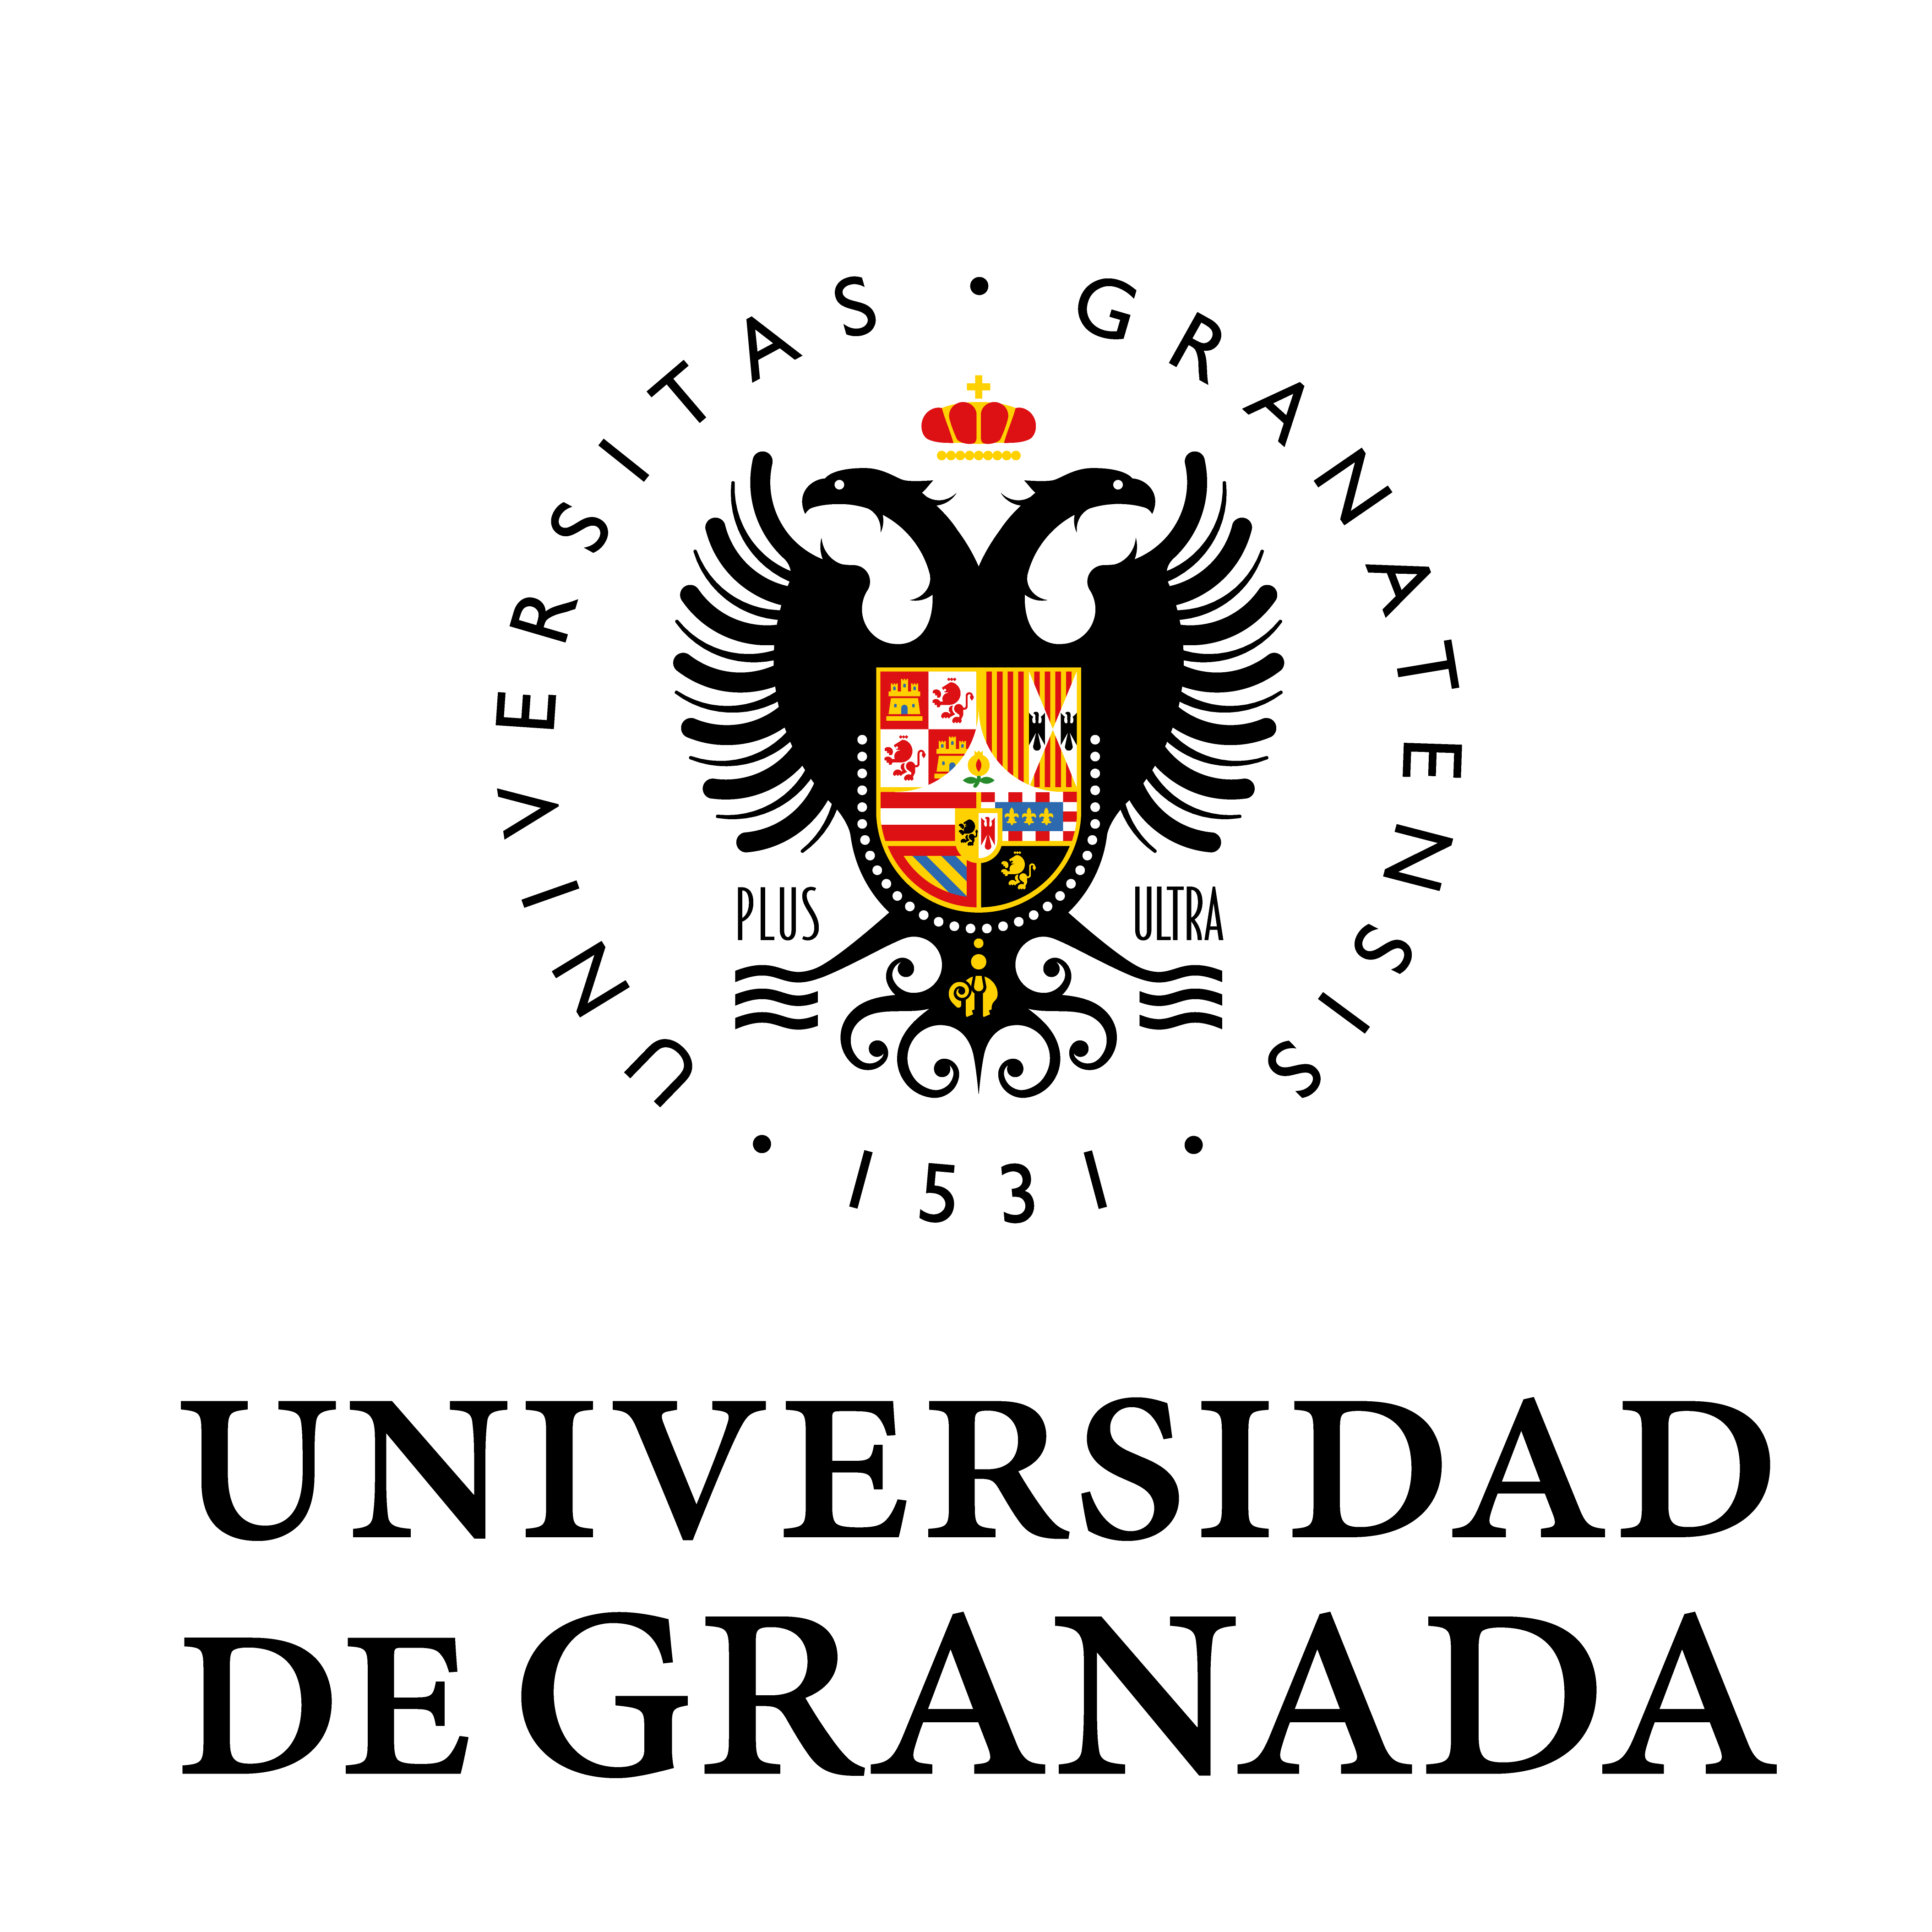
\includegraphics[width=0.6\textwidth]{ugr.png}\par\vspace{1cm}
  {\scshape\large Computación Ubicua e Inteligencia Ambiental \par} \vspace{1cm}
  {\huge\bfseries Desarrollo de aplicación de Realidad Aumentada \par}
  \vspace{0.4cm}
  {\large\itshape Modelos 3D interactivos para lápices 3D\\}
  \vspace{0.6cm}
  {\large\itshape  Nazaret Román Guerrero \\ Javier Sáez de la Coba  \par} \vspace{1.00cm}
  Curso 2018-2019 \\
  \vfill

  % Bottom of the page
  {\large \today\par}
\end{titlepage}

\tableofcontents
\newpage

\setlength{\parskip}{10pt}


\section{Descripción de la aplicación}
Nuestra idea es hacer una aplicación (a la que hemos llamado \textsc{modelos 3D interactivos para lápices 3D}) que vaya mostrando guías para ``pintar'' objetos tridimensionales con lápices 3D como el \emph{3Doodler}.
\begin{figure}[H]
    \centering
    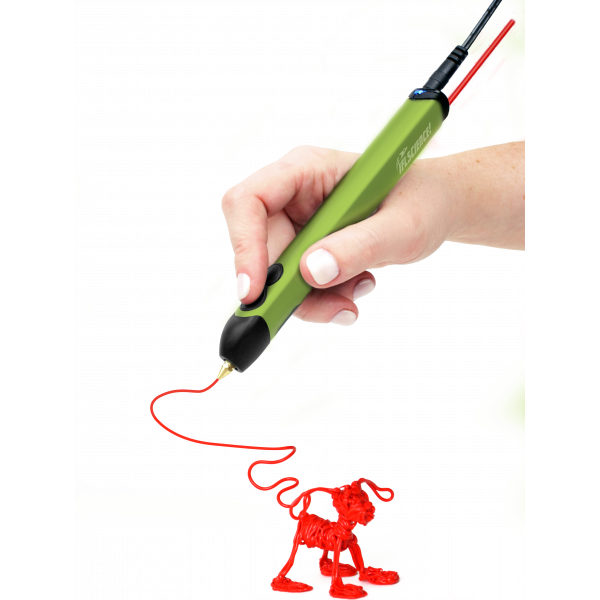
\includegraphics{3dpen.png}
    \caption{Lapiz 3D}
    \label{fig:my_label}
\end{figure}

En la aplicación que se va a desarrollar, la idea es que se pueda seleccionar entre varios modelos disponibles. Luego, sobre un tapete con marcadores se verá proyectado en tiempo real el modelo elegido que se desea construir. Con el lápiz 3D se irá formando  sobre el modelo hasta finalmente completarlo.

\section{Justificación/Motivación}
\subsection{Interés del problema a resolver}
Esta aplicación puede llegar a ser muy útil para aquellas personas que aún se estén iniciando en el uso de lápices 3D, ya que proporciona modelos que pueden ser fácilmente realizables con una ayuda visual como la que puede ofrecer la aplicación a desarrollar.

Puede ser útil, por ejemplo, para niños que quieran empezar a diseñar y construir objetos con esta herramienta, pero que aún no tienen una capacidad de diseño autónomo muy desarrollada y se ven obligados a utilizar una guía que los ayude en su construcción.

Otro sector al que puede estar orientado es en la educación. Es posible que en el futuro se puedan encontrar herramientas como los lápices 3D en las aulas de los colegios como una ayuda para desarrollar mejor disciplinas artísticas y a la vez introducir la tecnología desde edades tempranas. Por lo tanto, esta aplicación puede ayudar a los profesores y profesoras que impartan estas enseñanzas, haciendo más sencillo su aprendizaje mediante modelos virtuales de realidad aumentada.

Esta aplicación puede ser muy útil ya que, las aplicaciones disponibles actualmente que trabajan con lápices 3D, se basan en formar las piezas y más tarde unirlas (como se detalla un poco más en la sección \ref{competencia}). Con la aplicación que se va a diseñar lo que se pretende es crear directamente la estructura del modelo, no crear piezas independientes que luego sean ensambladas entre sí, lo que supone un avance en la manera de crear modelos con lápices 3D.

\subsection{Competencia} \label{competencia}

Actualmente la empresa 3Doodler ha creado una aplicación de planos para sus lápices 3D. En esta aplicación los planos aparecen en la pantalla de una tablet y consiste en dibujos planos. Estos dibujos luego se montan como si fueran piezas de un lego. La desventaja de esta aplicación es que no se hace el modelo completo, sino las partes separadas. En nuestra aplicación se tiene una visión global de como queda el modelo, la libertad de hacerlo desde cualquier orientación (moviendo la cámara o el tapete de marcadores) y la facilidad de ver el progreso de la construcción directamente.

\subsection{Opiniones de expertos, clientes y usuarios}
Para saber como sería acogida nuestra aplicación, preguntamos a unas pocas personas su opinión sobre la funcionalidad ofrecida. En el caso de que la mayoría de opiniones hubiesen sido negativas, habríamos cambiado el enfoque del funcionamiento de nuestra aplicación, puesto que es importante que los clientes y usuarios se sientan cómodos con una herramienta destinada a facilitarles el trabajo y no a complicarlo más.

\subsubsection{Expertos}
Los primeros a los que preguntamos fue a expertos, es decir, gente que trabaja o está directamente implicada con el diseño de lápices 3D y que está familiarizada con su uso, para poder tener una idea clara de si nuestra aplicación iba bien encaminada y podía tener futuro en el mercado. Hablamos con tres expertos, entre ellos, un familiar de uno de los creadores de la aplicación. Su intervención aclaro nuestras ideas a la hora de diseñar la aplicación para hacerla más cercana a los usuarios que finalmente la usen. Las opiniones son las que siguen:

\begin{itemize}
    \item \textit{``Lo primero en lo que tenéis que pensar es en los usuarios. Tenéis que hacer una interfaz amigable, y más aún si pretendéis que lo utilice gente que no está habituada a utilizar dispositivos electrónicos como son los niños''}.\\
    
    Es decir,  necesitamos hacer algo con lo que los usuarios se entiendan sin necesidad de tener una gran preparación de entornos informáticos, de manera que la interacción con la aplicación sea fácil e intuitiva.\\
    
    \item \textit{``Es importante la variedad de modelos, deberíais tener unos cuantos de cara a su salida al mercado. No vale que tenga pocos porque la gente se aburriría enseguida. Además, estaría bien si se pudiesen ir incorporando más modelos a la app según se deseara''}.\\
    
    Esta opinión nos dio una idea que podría ser bastante buena de cara a comercializar nuestra app. Si se introdujera algún tipo de IA que reconociese siluetas simples (no muy elaboradas puesto que con nuestra app solamente se crearía una estructura de alambres), podrían introducirse en la app nuevos modelos que desee cada usuario, es decir, si por ejemplo el usuario viaja a París y quiere diseñar un modelo de la torre Eiffel, solo tendría que enfocar dicho monumento y la IA podría crear un modelo simple que se guardaría en una base de datos y que podría servir para más usuarios en el futuro.\\
    
    \item \textit{``Necesitáis que la aplicación tenga soporte técnico y que sea multiplataforma. Así os aseguráis de que, en el caso de que los usuarios tengan algún problema, puedan contar con alguien que les ayude a solucionarlo y, al ser multiplataforma, también os aseguráis de que llega a un gran número de usuarios con dispositivos y softwares muy variados''}.\\
    
    A raíz de esto decidimos utilizar un software que diese pie a hacer una aplicación basada en web, ya que, por muy variados que sean los sistemas operativos o los dispositivos en los que se instale la app, todos disponen de un navegador a través del cual poder acceder a la aplicación sin necesidad de instalar software adicional que pudiese llevar a problemas de compatibilidad. Además, incluir un soporte nos proporciona un feedback sobre como está funcionando la aplicación y qué aspectos se pueden mejorar o qué funcionalidades se pueden añadir o eliminar.
\end{itemize}

\subsubsection{Clientes}
Hablamos con dos clientes para hacernos una idea de como se tomarían éstos comercialización de la app y cuáles eran sus principales exigencias. El segundo cliente al preguntamos también sería el usuario por lo que aparece también en la siguiente sección.

\begin{itemize}
    \item \textit{``Me gusta lo que se propone con la aplicación, pero me preocupa un poco que dependa de internet, puesto que yo tengo un niño pequeño al que me gustaría comprársela pero no me gusta que desde tan pequeño ya esté conectado a través de la red, ya que no sabes qué te puedes encontrar ahí y tendría que estar vigilado. Pero por lo demás me gusta bastante lo que proponéis, es muy útil y ayudaría a mi hijo a ser más creativo''}.\\
    
    Teniendo en cuenta lo que nos proponía este cliente, es cierto que el hecho de que fuese necesario una conexión a internet podría ser potencialmente peligroso para usuarios como el que se nos presenta en este caso, un niño de 9 años conectado en la red desde una temprana edad podría no ser exactamente lo que los padres desean. La solución que se nos planteó ante este problema fue crea una aplicación de escritorio o para un dispositivo como un móvil o una tablet que no requiera de conexión.\\
    
    \item \textit{``Me gusta la aplicación pero me preocupa que haya que pagar y después funcione mal. Hay aplicaciones de este tipo que hacen que me vaya muy lento el navegador y vaya} a tirones \textit{. Pero si va fluido y se ve bien, estaría encantado de utilizarla''}.\\
    
    Es importante hacer una aplicación funcional y eficiente que no vaya \textit{a tirones} como le preocupaba a este potencial cliente. Esto nos llevó a pensar que es necesario hacer una aplicación que funcione bien y que no requiera de un hardware demasiado avanzado o con grandes prestaciones, sino que funcione en un ordenador personal con una capacidad computacional nada extraordinaria.
\end{itemize}

\subsubsection{Usuarios}
En este caso, también hablamos con dos posibles usuarios, el hijo de nuestro cliente previo y el propio segundo cliente. El hecho de hablar con dos usuarios de edades dispares ayudó mucho a aclarar ideas que aún no estaban demasiado bien refinadas puesto que desde nuestro punto de vista como desarrolladores opinábamos una cosa que podía no adaptarse al gusto de los consumidores finales del software.

\begin{itemize}
    \item \textit{``Quiero que haya modelos como animales o coches para poder construirlos directamente con el lápiz.''}.\\
    
    Con ayuda del niño, nos dimos cuenta que es necesario incluir modelos que puedan ser atractivos para usuarios de edades jóvenes pero también para adultos, ya que distintos grupos de edades van a buscar modelos distintos, acordes a sus gustos.\\
    
    \item \textit{``Evidentemente, lo principal es que la aplicación se entienda bien y sea fácil de usar, y haya variedad de modelos con los que poder construir diferentes cosas. Creo que podría ser útil que tuviese un tutorial inicial para aprender a usarlo antes de construir modelos propiamente dichos''}.\\
    
    Al igual que el usuario anterior, éste desea cosas similares: gran variedad de modelos y que además, como nos dijo uno de los expertos, que sea una aplicación fácil de usar, intuitiva, que no dificultase la tarea del usuario. Además, la idea de un tutorial para aprender a construir un objeto simple como primer contacto con la aplicación está bien planteada, ya que podría ayudar a conseguir soltura utilizando el lápiz y la aplicación de forma que los controles se hicieran aún más sencillos si hay una guía previa que enseñe cómo usarlos.
\end{itemize}

\section{Hardware y Software a usar}
Queremos hacer la aplicación lo más multiplataforma posible. Para ello creemos que la mejor opción es hacer una aplicación basada en web usando las tecnologías de JavaScript y WebRTC que ofrecen los navegadores modernos. Esto nos permite que un usuario pueda usar la aplicación desde su ordenador con cámara web o desde su dispositivo móvil. 

El framework a usar (\textit{AR.js}) es compatible tanto con android como con iOS y con cualquier navegador de escritorio. Este framework de realidad aumentada está basado en marcadores. Hace uso de artoolkit y aruco como backends de detección y de three.js para la visualización de modelos 3D en un canvas usando WebGL.

Además su implementación como webapp permite establecer un sistema de logueo para que solo los usuarios autorizados utilicen la aplicación (escaneando el código de barras de su lápiz 3D). Como ventaja adicional, no ocupa espacio en el dispositivo y las actualizaciones y la adición de nuevos modelos se hace en el servidor (de forma transparente a los usuarios), y, por tanto, los clientes siempre disponen de la aplicación más actualizada. 

Como desventaja, la aplicación solo puede usarse disponiendo de una conexión a internet. Eso podemos resolverlo implementando la app como una webapp completa con posibilidad de funcionalidad offline. De esta forma los clientes solo tendrían que descargarse la aplicación la primera vez y funcionaría sin conexión. Aún así, presuponemos que los clientes tiene conectividad en principio, puesto que casi todo el mundo dispone de una conexión a internet estable y el uso de lápices 3D suele hacerse en entornos controlados y con conexión (hogar, oficina, colegios, etc).

Junto con \textit{AR.js} nos serviremos de otras tecnologías web estándar como bootstrap o flask para el desarrollo de la parte de la aplicación que no se refiere a la realidad aumentada (login, selección de modelos, configuración, etc).


\section{Informe de progreso (Entrega 2)}

\subsection{Aprendizaje del entorno}

El framework de \textit{AR.js} está basado en marcadores. Se puede utilizar únicamente un marcador, utilizar varios marcadores que den lugar a diferentes partes del modelo (el modelo se construye por piezas) o varios marcadores actuando como uno solo que den lugar al mismo modelo 3D.

Nosotros hemos optado por la tercera opción, ya que en el caso de que hay marcadores que se oculten parcialmente, hay otros marcadores alrededor (hay una malla) que podrán dar lugar al mismo modelo, aunque se hayan ocultado algunos. Es decir, hay marcadores de apoyo de forma que el modelo se siga visualizando.

A nivel técnico la aplicación consiste en una serie de archivos HTML que incluye a los scripts necesarios. Estos scripts hacen uso del estándar WebRTC para conseguir la imagen de la cámara del dispositivo en tiempo real. Luego mediante WebGL y una serie de librerías basadas en artoolkit procesa la imagen de la cámara con los marcadores y genera una escena 3D a integrar en la imagen de la cámara.

Además, existe otro HTML que se encarga de detectar por primera vez los marcadores y así generar un archivo de calibración.

El framework es bastante extenso, por lo que su aprendizaje no es tan sencillo como el de otros frameworks, sin embargo hace que la aplicación, al estar basada en estándares web, sea multiplataforma. Gracias a su gran librería de ejemplos se puede conseguir entender como funciona el sistema leyendo el código. 

\subsection{Prototipo de la aplicación}

Tras estudiar el framework, empezamos a ver sus posibilidades reales. Hemos ejecutado una demo en el ordenador portátil y hemos usado como marcadores un teléfono.

Tenemos pensado que el diseño final de la aplicación sea algo como lo siguiente, donde toda la parte azul claro se corresponde con lo que está grabando la cámara del ordenador y los botones se encuentran fijados sobre esa imagen:

\begin{figure}[H]
    \centering
        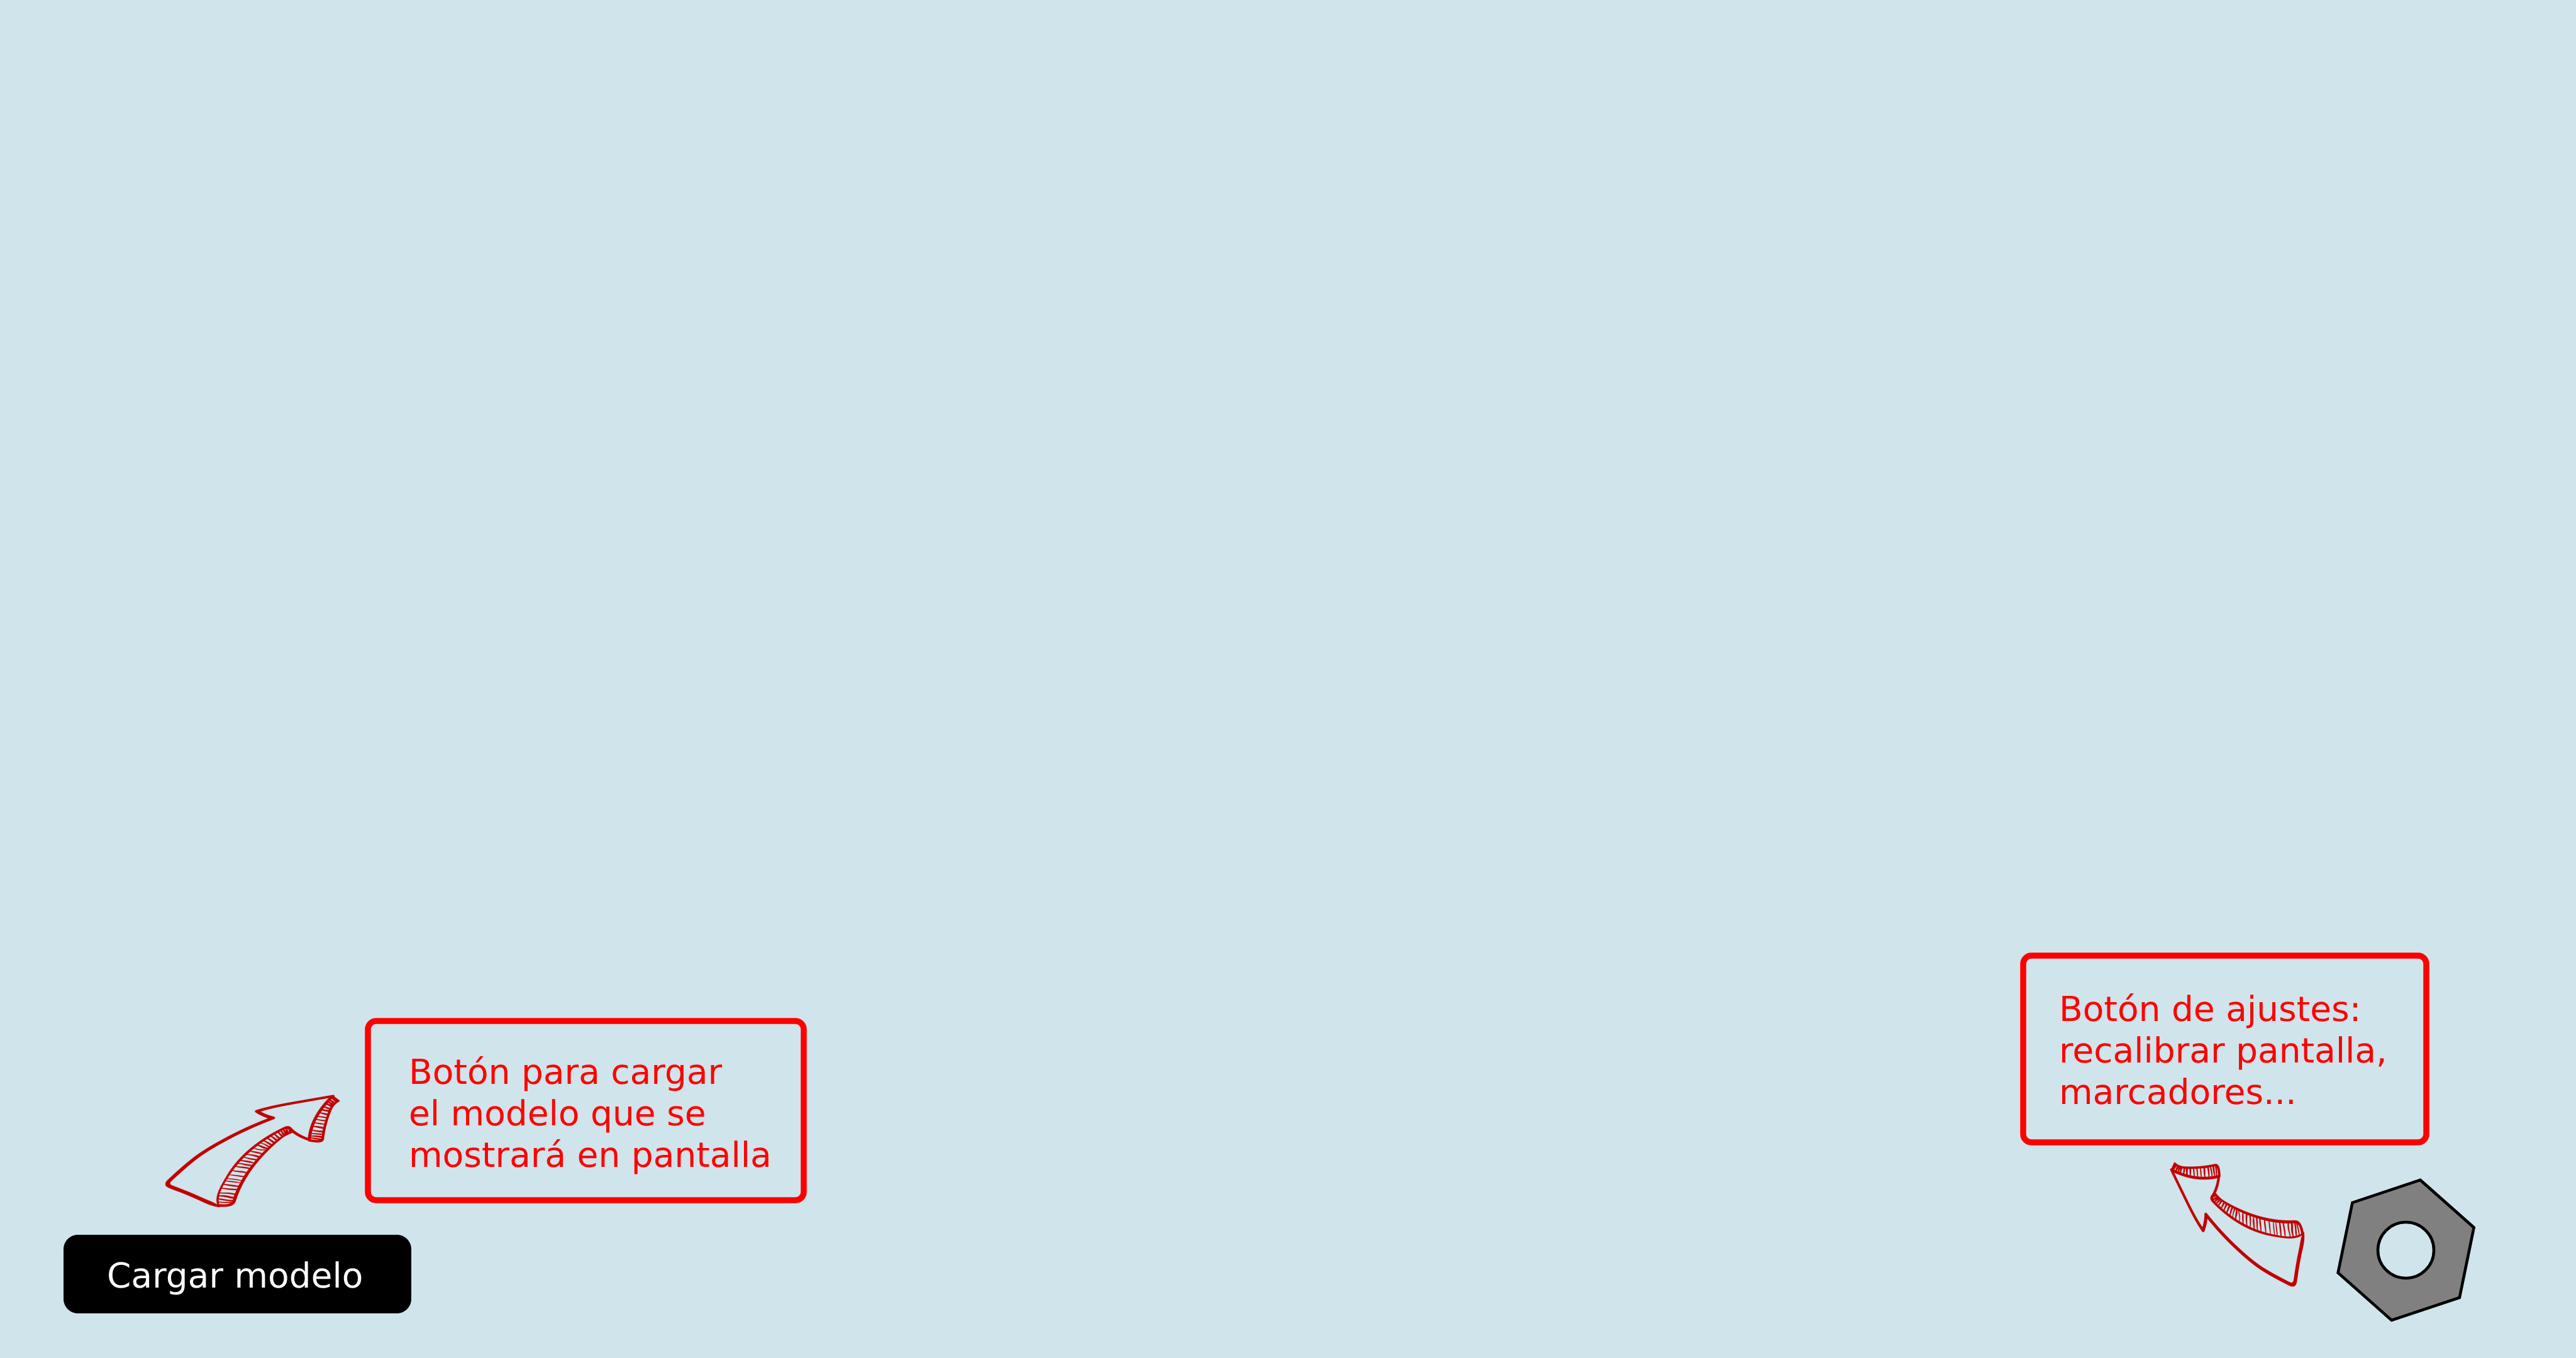
\includegraphics[width=0.8\textwidth]{proto.png}
        \caption{Prototipo de la aplicación}
        \label{fig:my_label}
\end{figure}

El diseño final se vería así:

\begin{figure}[H]
\centering
    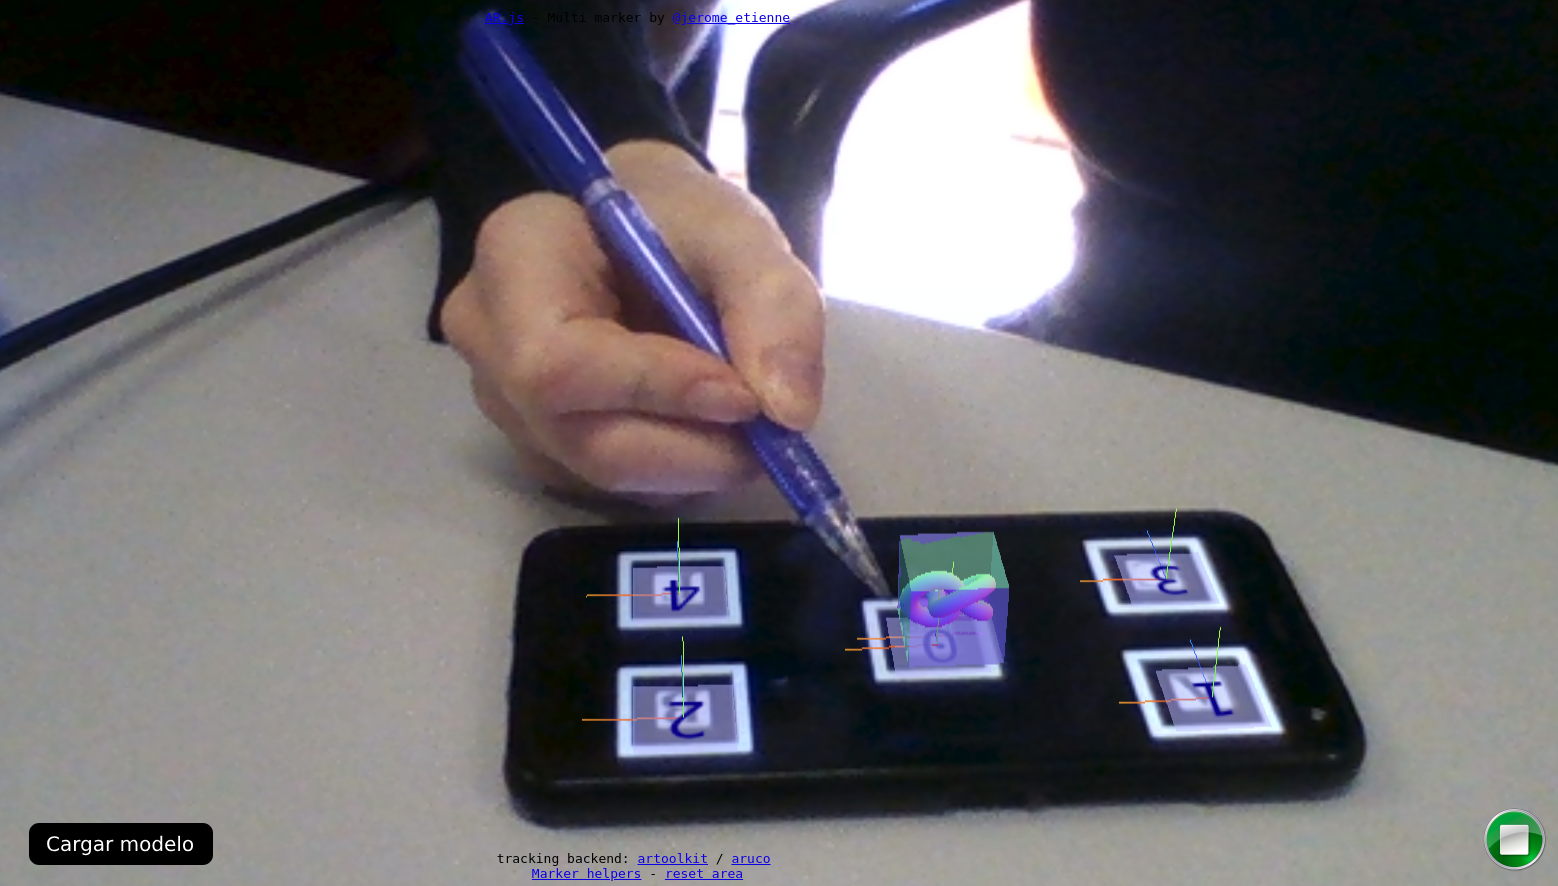
\includegraphics[width=0.8\textwidth]{fin_design.png}
    \caption{Demo básica del funcionamiento}
\end{figure}

\subsection{Descripción detallada de la aplicación}

Como cambios significativos con respecto a la práctica anterior, están los siguientes:

\begin{itemize}
    \item El nombre de nuestra aplicación ha sido cambiado ya que necesitábamos un nombre que llamara más la atención y atrajera a la gente; el nombre es \textit{\textbf{Air Draw}}.
\end{itemize}


\end{document}
